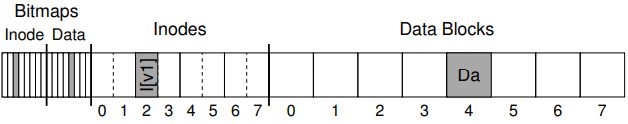
\includegraphics[width=\linewidth]{imgs/jn_eg1}
\begin{minipage}{.5\linewidth}
  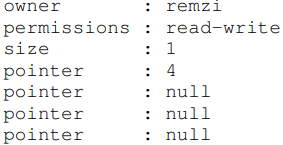
\includegraphics[width=\linewidth]{imgs/jn_eg3}
\end{minipage}
\begin{minipage}{.5\linewidth}
  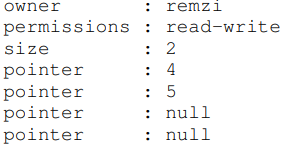
\includegraphics[width=\linewidth]{imgs/jn_eg4}
\end{minipage}
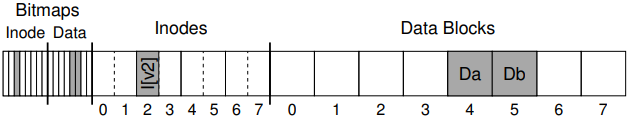
\includegraphics[width=\linewidth]{imgs/jn_eg2}
\begin{itemize}
\item assume workload: append 4KB data block to an existing file:
  \begin{enumerate*}[label={\arabic*.},font={\color{red!50!black}\bfseries}]
  \item \textrm{open()} file
  \item \texttt{lseek()} offset to file end
  \item \texttt{write()} 4KB and \texttt{close()} file
  \end{enumerate*}
\item assume simple filesys structs: 8-bit data bitmap (1/inode), 8-bit inode bitmap (1/data blk), 8 inodes (0-7, used 4 blks), 8 data blocks
\item 3 writes:
  \begin{enumerate*}[label={\arabic*.},font={\color{red!50!black}\bfseries}]
  \item the inode(I[v2])
  \item bitmap (B[v2])
  \item data blcok (Db)
  \end{enumerate*}
\item page/buffer cache keep data in RAM for a while before writing to disk
\item crash may occur between these 3 writes $\to$ file system in ? state
\item \mo{goal}: ensure at least the filesys is consistent; recover data if possible
\end{itemize}
\section*{Crash scenarios $\to$ inconsistent fs state, data loss, space leak}
\begin{tabular}{l|ccc|ll}
  S. & bitmaps   & inode     & [Db]      & fs         & user data \\
  \hline
  1  & \ding{55} & \ding{55} & \ding{51} & consistent   & lost$^{1}$\\
  2  & \ding{55} & \ding{51} & \ding{55} & inconsistent & inode \ding{220} garbage$^{2}$\\
  3  & \ding{51} & \ding{55} & \ding{55} & space leak$^{3}$ & blk5 never get used\\
  4  & \ding{51} & \ding{51} & \ding{55} & consistent & blk5 has garbage$^{2}$\\
  5  & \ding{55} & \ding{51} & \ding{51} & inconsistent & lost; recoverable \\
  6  & \ding{51} & \ding{55} & \ding{51} & inconsistent & belongs to no file\\
  \hline
  \multicolumn{6}{l}{1. as if the last write never occurred, fs OK, but user's data lost}\\
  \hline
  \multicolumn{6}{l}{2. blk 5 contains the old value before the write, thus garbage}\\
  \hline
  \multicolumn{6}{l}{3. fs inconsistent again, must resolve otherwise blk5 gets wasted}\\
  \hline
\end{tabular}
\section*{FileSys Check: make sure the fs metadata is internally consistent}
\begin{itemize}
\item Unix tool \texttt{fsck} is one example but tools can't fix all problems:
  \begin{enumerate*}[label={\arabic*.},font={\color{red!50!black}\bfseries}]
  \item can't recover lost data blocks if no inodes \ding{220} them
  \item can't tell whether a data block contains garbage
  \item only runs before fs mounted (see below)
  \end{enumerate*}
\item \textbf{superblock}:
  \begin{enumerate*}[label={\arabic*.},font={\color{red!50!black}\bfseries}]
  \item sanity checks: $S_{\text{fs}} \geq S_{\text{alloc}}$
  \item no corrupt superblock (use backup copy otherwise) \faStickyNoteO \texttt{fsck} \mr{scans entire fs and is too slow}
  \end{enumerate*}
\item \textbf{free} blocks:
  \begin{enumerate*}[label={\arabic*.},font={\color{red!50!black}\bfseries}]
  \item scan all inodes to collect allocated blocks $\to$ a correct version of allocation bitmaps and compare with bitmaps
  \item trust info within inodes $\to$ update bitmaps to be consistent with inodes
  \end{enumerate*}
\item \textbf{inode state}: check each inode for corruption or other problems:
  \begin{enumerate*}[label={\arabic*.},font={\color{red!50!black}\bfseries}]
  \item valid type: \texttt{-}, \texttt{d}, \texttt{l}
  \item clear corrupt inodes, update bitmap accordingly
  \end{enumerate*}
\item \textbf{inode links}: verify link/ref count of each allocated inode:
  \begin{enumerate*}[label={\arabic*.},font={\color{red!50!black}\bfseries}]
  \item scan entire dir tree; count link for each inode
  \item mismatch: trust the calculated link count
  \item put orphan (no entries \ding{220} it) to \texttt{lost+found} dir
  \end{enumerate*}
\item \textbf{duplicates}: check 2 inodes ref to same blk:
  \begin{enumerate*}[label={\alph*.},font={\color{red!50!black}\bfseries}]
  \item remove the obviously bad pointer
  \item copy data block so each inode has its own data
  \end{enumerate*}
\item \textbf{bad} blocks: check/clear ptrs \ding{220} sth outside valid range
\item \textbf{directory integrity checks}
  \begin{enumerate*}[label={\alph*.},font={\color{red!50!black}\bfseries}]
  \item \texttt{.}, \texttt{..} must be 1st entries
  \item each inode in an allocated dir
  \item each dir linked only once in entire tree hierarchy
  \end{enumerate*}
\end{itemize}
\section*{Journaling (or Write-Ahead Logging) - faster alternative}
\begin{minipage}{.5\linewidth}
  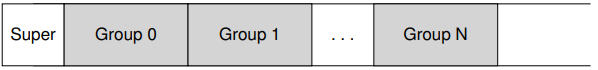
\includegraphics[width=\linewidth]{imgs/jn_ext2}
\end{minipage}
\begin{minipage}{.5\linewidth}
  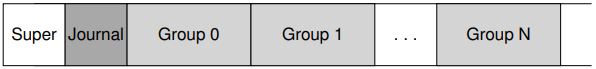
\includegraphics[width=\linewidth]{imgs/jn_ext3}
\end{minipage}
\begin{itemize}
\item Linux ext3 extends ext2 with journaling: small place on disk/other dev
\item basic idea:
  \begin{enumerate*}[label={\arabic*.},font={\color{red!50!black}\bfseries}]
  \item keep a note about what to write (log on a known disk location)
  \item commit the write as usual
  \item if crash, go back and check the note and retry (know exactly what to fix and how to fix)
  \end{enumerate*}
\item adds a bit extra work but greatly $\downarrow$ recovery workload (no scanning)
\end{itemize}
\begin{minipage}{.5\linewidth}
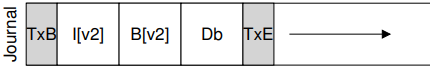
\includegraphics[width=\linewidth]{imgs/jn_dj1}
\end{minipage}
\begin{minipage}{.5\linewidth}
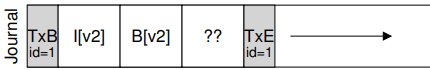
\includegraphics[width=\linewidth]{imgs/jn_dj2}
\end{minipage}
\begin{itemize}
\item TxB marks start of transaction: pretending update (to filesys) info I[v2], B[v2], DB; TxE the end; TID associated with TxB and TxE
\item middle 3 blocks contain exact block contents (physical logging)
\item checkpointing: once tx done, process of overwriting old structs on fs
\item sequence of operations:
  \begin{enumerate*}[label={\arabic*.},font={\color{red!50!black}\bfseries}]
  \item \textbf{journal write}: write TxB, inode, bitmap, data and TxE to the
journal; Wait for these writes to complete before proceeding
  \item \textbf{checkpoint}: Write the metadata (inode, bitmap) and data blocks to their final location
  \item what if a crash occurs during writing journal: (1) TxB, I[v2], B[v2], TxE and only later (2) Db
  \end{enumerate*}
\item tx looks valid: begin/end and ID; fs can't check for the wrong blk4
\item if reboot and recover, garbage copied to where Db supposed to live
\item bad for user data in a file; worse for fs superblock $\to$ unmountable
\end{itemize}
\begin{itemize}
\item ideal: write 5 blocks at once for a journal, yet unsafe $\because$ disk internally performs scheduling and complete parts of big writes in any order
\item simple but slow way: issue each write at time and wait for completion
\item real fs tx in 2 steps:
  \begin{enumerate*}[label={\arabic*.},font={\color{red!50!black}\bfseries}]
  \item writes all blks except TxE to journal at once and wait for completion
  \item issues write of TxE: in final, safe state
  \end{enumerate*}
\item write TxE must be atomic; disk guarantee any 512-byte write is atomic
\item one should make write of TxE a single 512-byte block
\end{itemize}
\begin{minipage}{.5\linewidth}
  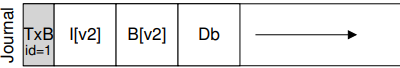
\includegraphics[width=\linewidth]{imgs/jn_dj3}
\end{minipage}
\begin{minipage}{.5\linewidth}
  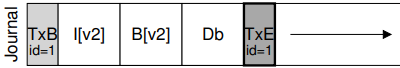
\includegraphics[width=\linewidth]{imgs/jn_dj4}
\end{minipage}
\begin{enumerate}
\item \textbf{journal write}: write the contents of the transaction (including TxB,
metadata, and data) to the log; wait for these writes to complete
\item \textbf{journal commit}: write tx commit block (containing
TxE) to the log; wait for write to complete; tx is said to be committed
\item \textbf{checkpoint}: write metadata and data blocks to their final location
\end{enumerate}
\section*{Recovery and Batch log updates}
\begin{itemize}
\item crash before \ml{2}: skip pending update, discard all tx without TxE
\item crash btwn \ml{2}-\ml{3}, recover the update as follow:
  \begin{enumerate*}[label={\alph*.},font={\color{red!50!black}\bfseries}]
  \item on sys boot, fs recovery process scans log for txs committed to disk
  \item replay such txs in order: retry writing blks in txs to their final on-disk locations (\mo{redo logging})
  \end{enumerate*}
\item crash any time in \ml{3}: fine; worst case: rewrite updates during recovery
\item journaling involves too many commits: some fs (ext3) buffer all updates into global tx (in RAM); write to disk later $\to$ disk traffic $\downarrow$
\end{itemize}
\section*{Making the log finite (circular log)}
\begin{minipage}{.45\linewidth}
  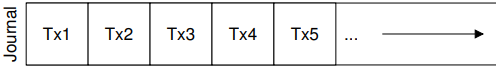
\includegraphics[width=\linewidth]{imgs/jn_logf1}
\end{minipage}
\begin{minipage}{.55\linewidth}
  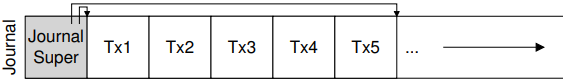
\includegraphics[width=\linewidth]{imgs/jn_logf2}
\end{minipage}
\begin{itemize}
\item the log/journal has fixed size: keep adding txs $\to$ log full and 2 problems:
  \begin{enumerate*}[label={\arabic*.},font={\color{red!50!black}\bfseries}]
  \item larger log $\to$ longer recovery $\because$ need to replay all txs in log
  \item no new txs can be committed to disk $\to$ \mo{updated protocol below}:
  \end{enumerate*}
\item
  \begin{enumerate*}[font={\color{lbl}\bfseries}]
  \item \textbf{journal write}: write contents of tx (TxB, metadata, and data) to log
  \item \textbf{journal commit}: write tx commit block (containing TxE) to log;
  \item \textbf{checkpoint}: write metadata and data blocks to their final location
  \item \textbf{free}: free ckpted txs in log; update journal superblock
  \end{enumerate*}
\item data journaling $\to$ write same blk \mr{twice} for each bitmap/data/inode
\item esp. painful during sequential write workload: 1/2 bandwidth only
\end{itemize}
\section*{Journaling Metadata only (aka ordered journaling of ext3)}
\begin{minipage}{.5\linewidth}
  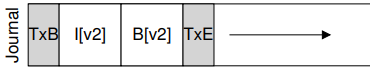
\includegraphics[width=\linewidth]{imgs/jn_mj1}
\end{minipage}
\begin{minipage}{.5\linewidth}
  \flushleft
  \begin{itemize}
  \item user data \emph{not} written to log $\to$ when to write it to disk?
  \item need to write user data \emph{first}
  \end{itemize}
\end{minipage}
\begin{itemize}
\item if Db written \emph{after} I[v2] \& B[v2], fs recovers garbage based on I[v2]
\item need to write Db \emph{first}, before I[v2]/B[v2] $\to$ updated protocol \faHandODown
\item
  \begin{enumerate*}[font={\color{lbl}\bfseries}]
  \item \textbf{data write}: write data to final location and wait for completion
  \item \textbf{journal metadata write}: write TxB, metadata to log; wait for completion
  \item \textbf{journal commit}: write tx commit block (containing TxE) to log;
  \item \textbf{checkpoint metadata}: write metadata to their final location in fs
  \item \textbf{free}: free ckpted txs in log; update journal superblock
  \end{enumerate*}
\item \ml{1} and \ml{2} can happen concurrently but must complete before \ml{3} starts
\end{itemize}
\section*{Tricky Case: Block Reuse}
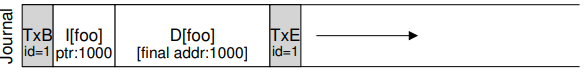
\includegraphics[width=\linewidth]{imgs/jn_tr1}
\begin{enumerate}
\item user adds a file entry to directory \texttt{foo} $\to$ content of \texttt{foo} written to log $\because$ directories are considered metadata; assume \texttt{foo} data at block 1000
\item user deletes all in \texttt{foo} (including itself); free up block 1000 for reuse
\item user creates new file \texttt{bar} that reuses same block 1000 $\to$ inode of \texttt{bar} committed to log: $\because$ metadata journaling is used in this case, only inode committed to journal, file \texttt{bar} \emph{not} journaled
\end{enumerate}
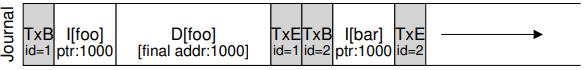
\includegraphics[width=\linewidth]{imgs/jn_tr2}
\begin{itemize}
\item assume a crash occurs, recovery process replays everything in log
\item overwrites user data of current \texttt{bar} with old directory contents!
\item deleting a dir/file \mo{won't} modify the logs about previous actions on it
\item possible solutions:
  \begin{enumerate*}[label={\arabic*.},font={\color{red!50!black}\bfseries}]
  \item never reuse blocks until the delete of said blocks is checkpointed out of the journal
  \item \faLinux ext3 adds  a new record type to journal: \textbf{revoke} record. In the case above, deleting the directory would cause a revoke record to be written to journal. When replaying the journal, fs first scans for such revoke records; any such revoked data is never replayed, thus avoiding the problem mentioned above.
  \end{enumerate*}
\end{itemize}
\begin{minipage}{.55\linewidth}
  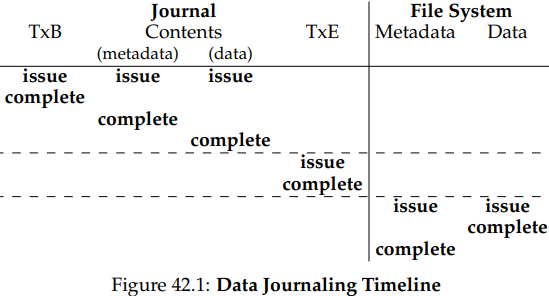
\includegraphics[width=\linewidth]{imgs/jn_tl1}
\end{minipage}
\begin{minipage}{.45\linewidth}
  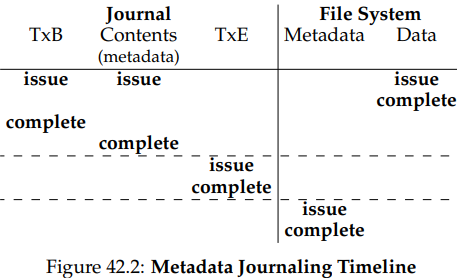
\includegraphics[width=\linewidth]{imgs/jn_tl2}
\end{minipage}
\begin{itemize}
\item each row shows logical time a write can be issued or may be complete
\item the time of completion marked for each write in timelines is arbitrary
\item in real system, completion time is determined by the I/O subsystem, which may reorder writes to improve performance
\item only guarantees about ordering: enforcement for protocol correctness
\item with a small checksum tweak, fs runs faster and more reliably \faHandODown
\end{itemize}
\begin{tcolorbox}[left=0mm, top=1mm, right=0mm, rightlower=0mm, bottom=1mm,
  title= \faLinux ext4 trick to optimize log writes,
  halign title=center]
  Include a checksum of the journal contents in begin/end blocks. Since checksum covers entire tx content, fs can write entire tx at once without a wait. If during recovery, the fs sees a mismatch in the computed checksum vs the stored one in the tx, it knows that a crash occurred during the tx write and thus discard the fs update
\end{tcolorbox}
